\chapter{Random Variables}

\section{Intro}


\begin{enumerate}
    \item A random variable is a numerical outcome of a random process.
    A random variable assigns a number to each possible outcome of a random experiment.
    \hfill \cite{common/online/chatgpt}

    \item An intuitive definition of a random variable or random quantity is a variable for which the value or outcome is unknown and for which the outcome is influenced by some form of random phenomenon.
    \hfill \cite{statistics/book/Statistics-for-Data-Scientists/Maurits-Kaptein}

    \item Why is it called "random"?
    Because the value it takes depends on chance.
    You don’t know the outcome in advance, but you know the possible values and can assign probabilities to them.
    \hfill \cite{common/online/chatgpt}

    \item This allows us to extend our theory on probability to other types of data without restricting it to specific events (i.e., binary data).
    \hfill \cite{statistics/book/Statistics-for-Data-Scientists/Maurits-Kaptein}

    \item The probability sampling approach makes the variable of interest a random variable, as the sampling approach is here the random phenomenon.
    \hfill \cite{statistics/book/Statistics-for-Data-Scientists/Maurits-Kaptein}

    \item A realization or an outcome of the random variable is then indicated by the same, but lower case, letter.
    \hfill \cite{statistics/book/Statistics-for-Data-Scientists/Maurits-Kaptein}

    \item a random variable may be seen as a variable that can in principle be equal to any of the values in the population, and after probability sampling the outcome(s) will become known.
    \hfill \cite{statistics/book/Statistics-for-Data-Scientists/Maurits-Kaptein}

    \item Types of Random Variables:
    \hfill \cite{common/online/chatgpt}
    \begin{enumerate}
        \item Discrete Random Variable:
        \hfill \cite{common/online/chatgpt}
        \begin{enumerate}
            \item Takes countable values (e.g., 0, 1, 2, 3…)
            \hfill \cite{common/online/chatgpt}

            \item Examples: number of heads in 10 coin tosses, number of emails received
            \hfill \cite{common/online/chatgpt}
        \end{enumerate}

        \item Continuous Random Variable
        \hfill \cite{common/online/chatgpt}
        \begin{enumerate}
            \item Takes uncountably many values in an interval (e.g., any real number)
            \hfill \cite{common/online/chatgpt}

            \item Examples: height of a person, temperature, time taken to run a race
            \hfill \cite{common/online/chatgpt}
        \end{enumerate}
    \end{enumerate}

    \item Notation:
    \begin{enumerate}
        \item Random variables are often written as capital letters like $X, Y, Z$
        \hfill \cite{common/online/chatgpt}

        \item Their values are written in lowercase, e.g., $X=x$
        \hfill \cite{common/online/chatgpt}
    \end{enumerate}

    \item The \textbf{probability function} $P(X \leq x)$ is a general concept and can be used for any random variable.
    \hfill \cite{statistics/book/Statistics-for-Data-Scientists/Maurits-Kaptein}

    \item The PMF for a discrete random variable is the equivalent of the PDF for a continuous random variable.
    \hfill \cite{statistics/book/Statistics-for-Data-Scientists/Maurits-Kaptein}

    \item Data points that are drawn independently from the same distribution ($D$ OR $D(\cdots)$) are said to be \textbf{independent and identically distributed}, which is often abbreviated to i.i.d. (denoted by $x \sim D$ OR $x \sim D(\cdots)$)
    \hfill \cite{ml/book/Pattern-Recognition-And-Machine-Learning/Christopher-M-Bishop}
\end{enumerate}





\section{Probability Density Functions (PDF) ($f(x) \neq P(X = x)$)}

\textbf{For Continuous Random Variable}

\begin{enumerate}
    \item The density function may be viewed as a smooth version of the histogram if we standardize the frequencies on the vertical axis to proportions.
    \hfill \cite{statistics/book/Statistics-for-Data-Scientists/Maurits-Kaptein}

    \item The density function characterizes the occurrence of values for a specific variable (as depicted on the x-axis) on all units from the population.
    \hfill \cite{statistics/book/Statistics-for-Data-Scientists/Maurits-Kaptein}

    \item Since in practice all populations are finite, the density function is an abstract formulation of, or a “model” for, the “frequencies” of all population values.
    \hfill \cite{statistics/book/Statistics-for-Data-Scientists/Maurits-Kaptein}

    \item PDF must satisfy two important conditions or properties:
    \hfill \cite{statistics/book/Statistics-for-Data-Scientists/Maurits-Kaptein}
    \begin{enumerate}
        \item  it cannot be negative, i.e., $f (x) \geq 0$ for every value $x$ that is present in the population
        For values of $x$ outside this domain, the PDF can then be defined equal to zero: $f (x) = 0$.
        \hfill \cite{statistics/book/Statistics-for-Data-Scientists/Maurits-Kaptein}

        \item  the “area under the curve” (AUC) is equal to one, i.e., $\dint_{\mbbR} f(x) dx = 1$
        \hfill \cite{statistics/book/Statistics-for-Data-Scientists/Maurits-Kaptein}
    \end{enumerate}

    \item Many different PDFs exist and they have been proposed over a period of more than two centuries to be able to describe populations and data in practical settings.
    \hfill \cite{statistics/book/Statistics-for-Data-Scientists/Maurits-Kaptein}
    \begin{enumerate}
        \item These functions are often parametric functions, i.e., the PDF is known up to a set of parameters.
        \hfill \cite{statistics/book/Statistics-for-Data-Scientists/Maurits-Kaptein}

        \item The PDF is then often denoted by $f_{\bm{\theta}}$ , where $\bm{\theta}$ represents the set or \textbf{vector} of $m$ density parameters:
        $\bm{\theta} =
        \begin{bmatrix}
            \theta_1 & \theta_2 & \cdots &\theta_m
        \end{bmatrix}
        ^\top
        $.
        \hfill \cite{statistics/book/Statistics-for-Data-Scientists/Maurits-Kaptein}
    \end{enumerate}

    \item  $f(x)$ is \textbf{not} be equal to $P(X = x)$
    \hfill \cite{statistics/book/Statistics-for-Data-Scientists/Maurits-Kaptein}
    \begin{enumerate}
        \item The probability $P(X = x)$ is equal to zero for continuous random variables, since there is no surface area under $f (x)$.
        \hfill \cite{statistics/book/Statistics-for-Data-Scientists/Maurits-Kaptein}
    \end{enumerate}
\end{enumerate}





\section{Probability Mass Function (PMF) ($f(x_k) = p_k = P(X = x_k)$)}

\textbf{For Discrete Random Variable}

\begin{enumerate}
    \item Discrete does not always mean that we observe values in $\mathbb{N}$.
    For instance, grades on a data science test may take values in $\dCurlyBrac{1, 1.5, 2.0, 2.5, \cdots , 9.0, 9.5, 10}$.
    Thus, it would be more rigorous to say that a discrete random variable $X$ takes its values in the set $\dCurlyBrac{x_0, x_1, x_2, \cdots , x _k , \cdots}$, with $x _k$ an element of the real line $(x _k \in \mbbR)$ and with an ordering of the values $x_0 < x_1 < x_2 < \cdots$ .
    However, in many practical settings we can map this set to a subset of $\mathbb{N}$ or to the whole set $\mathbb{N}$.
    \hfill \cite{statistics/book/Statistics-for-Data-Scientists/Maurits-Kaptein}

    \item For discrete random variables we can define $p _k = P(X = k)$ as the probability of observing the outcome $k$.
    \hfill \cite{statistics/book/Statistics-for-Data-Scientists/Maurits-Kaptein}

    \item This is referred to as the probability mass function (PMF) if the probabilities $p _k$ satisfy two conditions.
    \hfill \cite{statistics/book/Statistics-for-Data-Scientists/Maurits-Kaptein}
    \begin{enumerate}
        \item all probabilities $p _k$ should be nonnegative ( $p _k \geq 0, \forall\ k$)
        \hfill \cite{statistics/book/Statistics-for-Data-Scientists/Maurits-Kaptein}

        \item probabilities need to add up to one, i.e., $\dsum^{\infty}_{k=0} p _k = 1$
        \hfill \cite{statistics/book/Statistics-for-Data-Scientists/Maurits-Kaptein}
    \end{enumerate}
\end{enumerate}







\section{Cumulative Density Functions (CDF) ($F(x) = P(X \leq x)$)}

\subsection{Intro}

\begin{enumerate}
    \item The probability $P(X \leq x)$ is also referred to as the \textbf{distribution function} obtained in $x$ and it is denoted by $F(x) = P(X \leq x)$.
    Thus every random variable $X$ has a distribution function $F$ through $F(x) = P(X \leq x)$, but also every distribution function $F$ has a random variable $X$, namely the random variable $X$ that makes $P(X \leq x) = F(x)$.
    Thus the two concepts are directly related to each other and we then typically say that $X$ is distributed according to $F$, i.e., \colorbox{yellow}{$X \sim F$}.
    \hfill \cite{statistics/book/Statistics-for-Data-Scientists/Maurits-Kaptein}

    \item Each distribution function $F$ typically satisfies three conditions:
    \begin{enumerate}
        \item When the value $x$ increases to infinity, the distribution function becomes equal to one, i.e., $\lim _{x\to \infty} F(x) = 1$.
        \hfill \cite{statistics/book/Statistics-for-Data-Scientists/Maurits-Kaptein}

        \item When the value $x$ decreases to minus infinity the distribution function becomes equal to zero, i.e., $\lim _{x\to -\infty} F(x) = 0$.
        \hfill \cite{statistics/book/Statistics-for-Data-Scientists/Maurits-Kaptein}

        \item The distribution function is a non-decreasing function, i.e., $F(x_1) \leq F(x_2)$ when $x_1 \leq x_2$.
        \hfill \cite{statistics/book/Statistics-for-Data-Scientists/Maurits-Kaptein}
    \end{enumerate}


\end{enumerate}


\subsection{CDF of PDF (Continuous)}


\begin{enumerate}
    \item There is a direct relation between distribution functions and densities.
    If we start with a PDF, we can define a distribution function in the following way:
    \colorbox{yellow}{$
        F(x)
        = P(X \leq x)
        = \dint_{-\infty}^{x} f(z) dz
    $}
    \hfill \cite{statistics/book/Statistics-for-Data-Scientists/Maurits-Kaptein}

    \item The full distribution function of $\psi(X)$ can always be established, but it does not always have a simple workable form.
    \hfill \cite{statistics/book/Statistics-for-Data-Scientists/Maurits-Kaptein}
    \\[0.2cm]
    $
        P(\psi^{-1}(X) \leq x)
        = P(X \leq \psi(x))
        = F(\psi(x))
        =\dint_{-\infty}^{\psi(x)} f(z) dz
        =\dint_{-\infty}^{x} \psi^{\prime}(z)\ f(\psi(z))\ dz
    $
    \hfill \cite{statistics/book/Statistics-for-Data-Scientists/Maurits-Kaptein}
    \\[0.2cm]
    The calculations now show that the distribution function of random variable $\psi^{-1}(X)$ is equal to $F(\psi(x))$ and the PDF is $\psi^\prime(x)\ f (\psi(x))$.
    \hfill \cite{statistics/book/Statistics-for-Data-Scientists/Maurits-Kaptein}
    \\[0.5cm]
    \textbf{Example}: Let $X$ being normally distributed with parameters $\mu$ and $\sigma$, and consider the function $\psi(x) = \exp\dCurlyBrac{x}$
    \hfill \cite{statistics/book/Statistics-for-Data-Scientists/Maurits-Kaptein}
    \\[0.2cm]
    $
        P(X \leq x)
        = \dint_{-\infty}^{x} \dfrac{1}{\sigma} \phi\dParenBrac{\dfrac{z - \mu}{\sigma}}
        = \dint_{-\infty}^{(x - \mu)/\sigma} \phi(z)\ dz
        = \Phi\dParenBrac{\dfrac{x - \mu}{\sigma}}
    $
    \hfill \cite{statistics/book/Statistics-for-Data-Scientists/Maurits-Kaptein}
    \\[0.2cm]
    $
        \begin{aligned}
            P(\exp\dCurlyBrac{X} \leq x)
                &= P(X \leq \log(x))
                = \Phi\dParenBrac{\dfrac{\log(x) - \mu}{\sigma}} \\
                &= \dint_{-\infty}^{\log(x)} \dfrac{1}{\sigma} \phi\dParenBrac{\dfrac{z - \mu}{\sigma}} dz
                = \dint_{0}^{x} \dfrac{1}{z\sigma} \phi\dParenBrac{\dfrac{\log(z) - \mu}{\sigma}} dz
        \end{aligned}
    $
    \hfill \cite{statistics/book/Statistics-for-Data-Scientists/Maurits-Kaptein}






    \item $P(X < x) = P(X \leq x)$ for continuous random variables

    \item $P(X > x) = 1 - P(X \leq x)$
    \hfill \cite{statistics/book/Statistics-for-Data-Scientists/Maurits-Kaptein}

    \item $P( x_1 < X \leq x_2) = P(X \leq x_2) - P(X \leq x_1)$
    \hfill \cite{statistics/book/Statistics-for-Data-Scientists/Maurits-Kaptein}
\end{enumerate}



\subsection{CDF of PMF (Discrete)}

\begin{enumerate}
    \item The distribution function or cumulative density function (CDF) for a discrete random variable $X$ is now given by \colorbox{yellow}{$F(x) = P(X \leq x) = \dsum^{x}_ {k=0} f (k)$}.
    \hfill \cite{statistics/book/Statistics-for-Data-Scientists/Maurits-Kaptein}

    \item If the set is $\dCurlyBrac{x_0, x_1, x_2, \cdots , x _k , \cdots}$, with $x_0 < x_1 < x_2 < \cdots$ , then the CDF is defined as \colorbox{yellow}{$F(x) =\dsum^{m_x} _{k=0} f (x _k )$}, with $m _x$ the largest value for $k$ that satisfies $x_ k \leq x$.
    \hfill \cite{statistics/book/Statistics-for-Data-Scientists/Maurits-Kaptein}
\end{enumerate}




\section{Expected Values ($E(X)$)}

\subsection{For PDF (Continuous)}

\begin{enumerate}
    \item If we consider a (not necessarily continuous or differentiable) function $\psi : \mbbR \to \mbbR$, then the expected value of the random variable $\psi (X)$ is defined by
    \colorbox{yellow}{$
        \mbbE[\psi(X)]
        = \dint_{\mbbR} \psi(x)\ f(x)\ dx
    $}
    \hfill \cite{statistics/book/Statistics-for-Data-Scientists/Maurits-Kaptein}
\end{enumerate}

\subsection{For PMF (Discrete)}

\begin{enumerate}
    \item The expectation of a discrete random variable $\psi(X)$ is given by
    \hfill \cite{statistics/book/Statistics-for-Data-Scientists/Maurits-Kaptein}
    \\[0.2cm]
    \colorbox{yellow}{$
        \mbbE[\psi(X)] \
        = \dsum^{\infty}_{k=0}\ \psi(k)\ p _k \
        = \dsum^{\infty}_{k=0}\ \psi(k)\ P(X = k)
    $}
    \hfill \cite{statistics/book/Statistics-for-Data-Scientists/Maurits-Kaptein}

    \item If we would collect many realizations of the discrete random variable $X$, say $N$ realizations, we expect to see value $k$ with frequency $N \cdot p _k$ .
    \hfill \cite{statistics/book/Statistics-for-Data-Scientists/Maurits-Kaptein}
\end{enumerate}

\subsection{Common for PDF \& PMF}

\begin{enumerate}
    \item \textbf{First moment}: mean $\mu$ is obtained by \colorbox{yellow}{$\psi(x)=x$}
    \hfill \cite{statistics/book/Statistics-for-Data-Scientists/Maurits-Kaptein}

    \item \textbf{Second central moment}: The population variance $\sigma^ 2$ is obtained by \colorbox{yellow}{$\psi(x)=(x -\mu)^2$}
    \hfill \cite{statistics/book/Statistics-for-Data-Scientists/Maurits-Kaptein}

    \item \textbf{pth moment} of random variable $X$ is obtained by \colorbox{yellow}{$\psi(x) = x^p$}
    \hfill \cite{statistics/book/Statistics-for-Data-Scientists/Maurits-Kaptein}

    \item \textbf{pth central moment} of random variable $X$ is obtained by choosing \colorbox{yellow}{$\psi(x) = (x - \mu)^p$}
    \hfill \cite{statistics/book/Statistics-for-Data-Scientists/Maurits-Kaptein}

    \item \textbf{skewness}: \colorbox{yellow}{$\gamma_1 = \dfrac{\mu_3}{\sigma^3}$}, where $\mu_3 = \mbbE[(x-\mu)^3]$
    \hfill \cite{statistics/book/Statistics-for-Data-Scientists/Maurits-Kaptein}

    \item \textbf{kurtosis}: \colorbox{yellow}{$\gamma_2 = \dfrac{\mu_4}{\sigma^4} - 3$}, where $\mu_4 = \mbbE[(x-\mu)^4]$
    \hfill \cite{statistics/book/Statistics-for-Data-Scientists/Maurits-Kaptein}
\end{enumerate}

\vspace{0.5cm}
\textbf{Note}:
\begin{enumerate}
    \item the moments of a discrete random variable $X$ may \textbf{not} always exist: this depends on the choice of probabilities $p _k $.
    \hfill \cite{statistics/book/Statistics-for-Data-Scientists/Maurits-Kaptein}
\end{enumerate}


\section{Calculation Rules for Random Variables}

Let we have 2 random variables $X, \ Y$, either discrete or continuous, and a constant $c$.
\\
$F _X$ and $F_Y$ the CDFs for $X$ and $Y$ , respectively. $P(X \leq x, Y \leq y)$ is the joint CDF
of $X$ and $Y$ , denoted by $F _{X Y} (x, y)$
\\
Let events $A = \dCurlyBrac{X \leq x}$ and $B = \dCurlyBrac{Y \leq y}$

\begin{multicols}{2}
\begin{enumerate}[series=calcrulesrv]
    \item $\mbbE[c] = c$
    \hfill \cite{statistics/book/Statistics-for-Data-Scientists/Maurits-Kaptein}

    \item $\mbbE[cX] = c \mbbE[X]$
    \hfill \cite{statistics/book/Statistics-for-Data-Scientists/Maurits-Kaptein}

    \item $\text{Var}[X] \geq 0$
    \hfill \cite{statistics/book/Statistics-for-Data-Scientists/Maurits-Kaptein}

    \item $\text{Var}[X + c] = \text{Var}[X]$
    \hfill \cite{statistics/book/Statistics-for-Data-Scientists/Maurits-Kaptein}

    \item $\text{Var}[cX] = c^2\ \text{Var}[X]$
    \hfill \cite{statistics/book/Statistics-for-Data-Scientists/Maurits-Kaptein}

    \item $\text{Var}[X] = \mbbE[X^2] - (\mbbE[X])^2$
    \hfill \cite{statistics/book/Statistics-for-Data-Scientists/Maurits-Kaptein}

    \item $\mbbE[X] = \mbbE[Y]$ , when $X = Y$
    \hfill \cite{statistics/book/Statistics-for-Data-Scientists/Maurits-Kaptein}

    \item $\mbbE[X + Y] = \mbbE[X] + \mbbE[Y]$
    \hfill \cite{statistics/book/Statistics-for-Data-Scientists/Maurits-Kaptein}
\end{enumerate}
\end{multicols}

\textbf{if $X$ and $Y$ are independent:}

\begin{multicols}{2}
\begin{enumerate}[resume*=calcrulesrv]
    \item $\phi(X)$ and $\psi(Y)$ are also independent
    \hfill \cite{statistics/book/Statistics-for-Data-Scientists/Maurits-Kaptein}

    \item $\mbbE[X Y]  = \mbbE[X]\ \mbbE[Y]$
    \hfill \cite{statistics/book/Statistics-for-Data-Scientists/Maurits-Kaptein}

    \item $\tVar[X \pm Y] = \tVar[X] + \tVar[Y]$
    \hfill \cite{statistics/book/Statistics-for-Data-Scientists/Maurits-Kaptein}

\end{enumerate}
\end{multicols}


\begin{enumerate}[resume*=calcrulesrv]
    \item
    $
        P(X \leq x, Y \leq y)
        = P(A \cap B)
        = P(A) P(B)
        = P(X \leq x) P(Y \leq y)
        = F _X (x)\ F_Y (y)
    $
    \hfill \cite{statistics/book/Statistics-for-Data-Scientists/Maurits-Kaptein}

    \item
    $
        \text{Var}[X Y]
        = \text{Var}[X] \text{Var}[Y]
            + \text{Var}[X](\mbbE[Y])^2
            + \text{Var}[Y](\mbbE[X])^2
    $
    \hfill \cite{statistics/book/Statistics-for-Data-Scientists/Maurits-Kaptein}
\end{enumerate}



\section{Sample Statistics ($T_n$), Estimators \& Summary Statistics}


\begin{figure}[H]
    \centering
    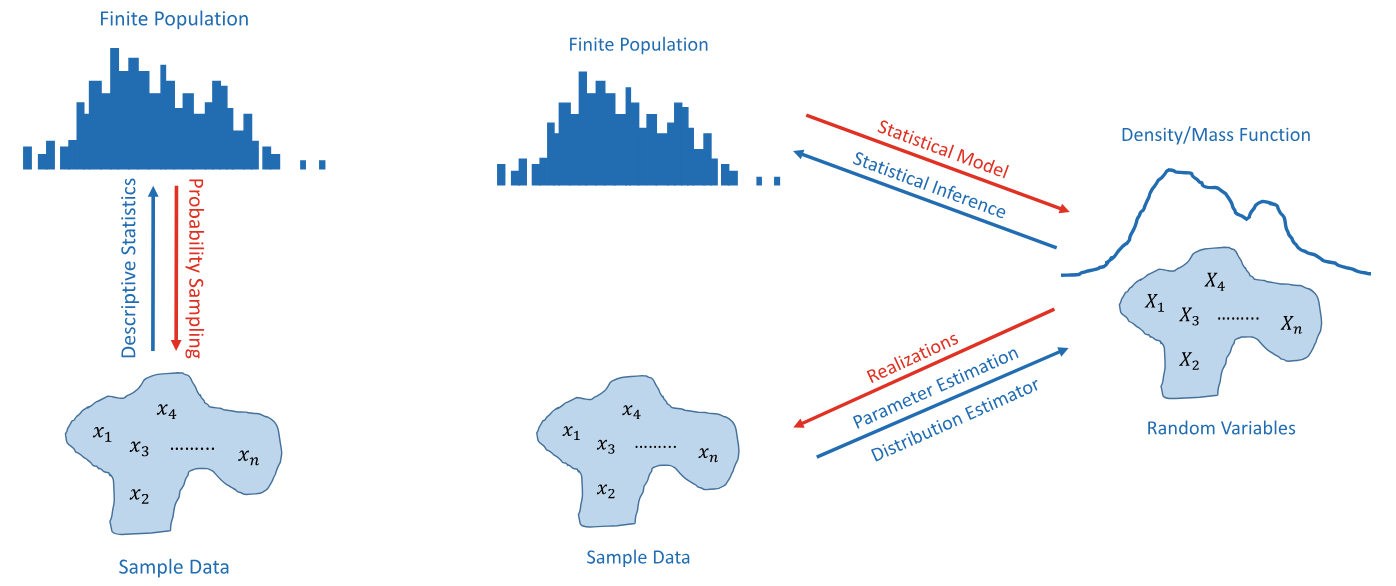
\includegraphics[
        width=\linewidth,
        height=5cm,
        keepaspectratio,
    ]{images/statistics/population-statistics-estimation.png}
    \caption*{
        we use the theory of random variables and distribution functions allows us to make more detailed statements about the population of interest
        \cite{statistics/book/Statistics-for-Data-Scientists/Maurits-Kaptein}
    }
\end{figure}


\begin{enumerate}
    \item Sample statistics are numerical values calculated from a sample (a subset of a population) to describe some aspect of the sample.
    \hfill \cite{common/online/chatgpt}

    \item An \textbf{estimator} is a rule or formula (usually a function of sample data) used to estimate a population parameter.
    \hfill \cite{common/online/chatgpt}

    \item These are statistics that summarize or describe features of a dataset.
    They can be from either a sample or an entire population.
    \hfill \cite{common/online/chatgpt}

    \item We are often interested in summarizing sets of random variables and comparing pairs of random variables.
    \hfill \cite{mfml/book/mml/Deisenroth-Faisal-Ong}

    \item A \textbf{statistic of a random variable} is a deterministic function of that random variable.
    \hfill \cite{mfml/book/mml/Deisenroth-Faisal-Ong}

    \item The summary statistics of a distribution provide one useful view of how a random variable behaves, and provides numbers that summarize and characterize the distribution.
    \hfill \cite{mfml/book/mml/Deisenroth-Faisal-Ong}

    \item Going from the data to the PDF or PMF to the population is also called statistical inference, but now we are using (parametric) statistical models.
    \hfill \cite{statistics/book/Statistics-for-Data-Scientists/Maurits-Kaptein}

    \item \textbf{Population Characterstics}:
    \begin{enumerate}
        \item \textbf{standardized variable};
        $
            Z = \dfrac{X - \mu( f )}{\sigma ( f )}
        $
        \hfill \cite{statistics/book/Statistics-for-Data-Scientists/Maurits-Kaptein}

        \item \textbf{population mean}:
        $
            \mu  ( f )
            = \mbbE[X]
            = \dint _\mbbR x f (x)dx
        $
        \hfill \cite{statistics/book/Statistics-for-Data-Scientists/Maurits-Kaptein}

        \item \textbf{population variance}:
        $
            \sigma ^2 ( f )
            = \mbbE [(X - \mu ( f ))^2]
            = \dint _\mbbR (x - \mu ( f ))^2 f (x) dx
        $
        \hfill \cite{statistics/book/Statistics-for-Data-Scientists/Maurits-Kaptein}

        \item \textbf{population standard deviation}:
        $
            \sigma ( f )
            = \sqrt{\sigma ^2 ( f ) }
        $
        \hfill \cite{statistics/book/Statistics-for-Data-Scientists/Maurits-Kaptein}

        \item \textbf{Third moment (skewness)}:
        $
            \gamma_1( f ) = \mbbE [(Z )^3]
        $
        \hfill \cite{statistics/book/Statistics-for-Data-Scientists/Maurits-Kaptein}

        \item \textbf{Fourth moment (excess kurtosis)}:
        $
            \gamma_2( f ) = \mbbE [(Z )^4]-3
        $
        \hfill \cite{statistics/book/Statistics-for-Data-Scientists/Maurits-Kaptein}

        \item \textbf{Quantiles}:
        $
            F (x _p ( f )) = \dint ^{x _p ( f )} _{-\infty} f (x) dx = p
            \Rightarrow
            x _p ( f ) = F^{-1} ( p)
        $
        \hfill \cite{statistics/book/Statistics-for-Data-Scientists/Maurits-Kaptein}
        \\
        $F^{-1}$ is the inverse distribution function
        \hfill \cite{statistics/book/Statistics-for-Data-Scientists/Maurits-Kaptein}

        \item [\textbf{Note}:] we are now using the notation $\mu ( f )$ to make explicit that the population mean $\mu$ will depend on our choice of $f$ .
        \hfill \cite{statistics/book/Statistics-for-Data-Scientists/Maurits-Kaptein}
    \end{enumerate}
\end{enumerate}





\subsection{Distributions of Sample Statistic $T_n$}


\begin{enumerate}
    \item \textbf{PMF or PDF}
    \hfill \cite{statistics/book/Statistics-for-Data-Scientists/Maurits-Kaptein}
    \begin{enumerate}
        \item In many settings, the sample distribution function has a sample PMF or PDF $f _{T_n}$ , often referred to as the sample density function of $T_n$ .
        \hfill \cite{statistics/book/Statistics-for-Data-Scientists/Maurits-Kaptein}

        \item  it is not always easy to determine the sample distribution or sample density function in general
        \hfill \cite{statistics/book/Statistics-for-Data-Scientists/Maurits-Kaptein}

        \item Only in special cases is it possible to determine closed-form functions.
        \hfill \cite{statistics/book/Statistics-for-Data-Scientists/Maurits-Kaptein}
    \end{enumerate}

    \item \textbf{CDF}: $F_{T_n} (x) = P (T_n \leq x)$
    \hfill \cite{statistics/book/Statistics-for-Data-Scientists/Maurits-Kaptein}
    \begin{enumerate}
        \item This CDF is often referred to as the sample distribution function of statistic $T_n$ , as it describes how the sample statistics vary if we draw (new) samples from the population.
        \hfill \cite{statistics/book/Statistics-for-Data-Scientists/Maurits-Kaptein}

    \end{enumerate}

    \item We study the distributions of $T_n$, as these distribution functions effectively allow us to examine the quality of our estimators: the distribution function of the random variable $T_n$ provides a measure of how well an estimator approximates a population value.
    \begin{enumerate}
        \item The expected value of an estimator $\mbbE[T_n]$ is a measure for the central tendency of a sample statistic
        \hfill \cite{statistics/book/Statistics-for-Data-Scientists/Maurits-Kaptein}

        \item The standard deviation of $T_n$ provides a measure for the variability of a sample statistic.
        The standard deviation of a sample statistic $T_n$ is the standard error of that sample statistic;
        the standard error of a sample statistic of interest is commonly reported in scientific texts to quantify the uncertainty associated with the sample statistic.
        \hfill \cite{statistics/book/Statistics-for-Data-Scientists/Maurits-Kaptein}
    \end{enumerate}
\end{enumerate}


\subsubsection{Distribution of the Sample Minimum}

\begin{enumerate}
    \item $F _{X_{(1)}}(x) = 1 - [1 - F(x)]^n$
    \hfill \cite{statistics/book/Statistics-for-Data-Scientists/Maurits-Kaptein}

    \item $f _{X_{(1)}} (x) = n [1 - F(x)]^{n-1}\ f (x)$
    \hfill \cite{statistics/book/Statistics-for-Data-Scientists/Maurits-Kaptein}
\end{enumerate}

\subsubsection{Distribution of the Sample Maximum}

\begin{enumerate}
    \item  Let $T_n$ be the maximum of $X_1 , X_2, \cdots , X _n$ , the distribution function of $T_n$ is given by:
    \hfill \cite{statistics/book/Statistics-for-Data-Scientists/Maurits-Kaptein}
    \\
    $
        \begin{aligned}
            F _{X_{(n)}} (x)
            &= P (X_{(n)} \leq x)
            = P (\max \dCurlyBrac{X_1, X_2, \cdots, X _n } \leq x) \\
            &= P (X_1 \leq x, X_2 \leq x, \cdots, X _n \leq x)
            = \dprod ^n _{i=1} P (X _i \leq x)
            = \dprod ^n _{i=1} F(x) \\
            &= [F (x)]^n
        \end{aligned}
        \hfill \text{\cite{statistics/book/Statistics-for-Data-Scientists/Maurits-Kaptein}}
    $

    \item $f _{X_{(n)}} (x) = n [F (x)]^{n-1}\ f (x)$
    \hfill \cite{statistics/book/Statistics-for-Data-Scientists/Maurits-Kaptein}
\end{enumerate}



\subsubsection{Distribution of the Sample Average}

\begin{enumerate}
    \item The distribution function of the sample average $\bar{X} = \dfrac{1}{n} \dsum^n _{i=1} X _i$ is not so easy to determine in general.
    \hfill \cite{statistics/book/Statistics-for-Data-Scientists/Maurits-Kaptein}

    \item The $p$-th moment of a general sample statistic $T_n$ is given by
    $\mbbE[T ^p _n] = \dint _\mbbR t^ p f _{T_n} (t) dt$,
    if the sample density $f _{T_n}$ exists, using the definition of moments for any random variable.
    \hfill \cite{statistics/book/Statistics-for-Data-Scientists/Maurits-Kaptein}

    \item  It can, however, also be calculated in a different way, using the population density $f$ and the fact that $X_1 , X_2, \cdots , X _n$ are i.i.d. $F$.
    The $p$-th moment of $T_n$ is:
    \hfill \cite{statistics/book/Statistics-for-Data-Scientists/Maurits-Kaptein}
    \\
    .\hfill
    $
        \begin{aligned}
            \mbbE[T ^p _n]
            &= \dint _\mbbR t ^p f_ {T_n} (t) dt
            = \mbbE[T ^p _n (X_1, X_2, \cdots , X _n )] \\
            &= \dint _{\mbbR^n} T ^p _n (x_1, x_2, \cdots , x _n )\ f (x_1) f (x_2) \cdots f (x _n ) \ dx_1dx_2 \cdots dx _n
        \end{aligned}
    $
    \hfill \cite{statistics/book/Statistics-for-Data-Scientists/Maurits-Kaptein}

    \item A special case is the first moment $\mu ( f_ {T_n} ) = \mbbE[T_n]$
    \hfill \cite{statistics/book/Statistics-for-Data-Scientists/Maurits-Kaptein}

    \item The advantage of $\mbbE[T ^p _n]$ equation is that the moments of the sample statistic $T_n = \bar{X}$ can be expressed in moments of the random variables $X_1 , X_2, \cdots , X _n$.
    Indeed, the first moment of $\bar{X}$ is now given by
    \hfill \cite{statistics/book/Statistics-for-Data-Scientists/Maurits-Kaptein}
    \\[0.3cm]
    .\hfill
    $
        \begin{aligned}
            \mu ( f _{\bar{X}} )
            &= \mbbE[\bar{X}]
            = \dint _{\mbbR^n} \dParenBrac{\dfrac{1}{n} \dsum ^n _{i=1} x_ i }\ f (x_1) f (x_2) \cdots f (x _n )\ dx_1dx_2 \cdots dx _n \\
            &= \dfrac{1}{n} \dsum^n _{i=1} \dint _{\mbbR^n} x _i\ f (x_1) f (x_2) \cdots f (x_ n )\ dx_1dx_2 \cdots dx _n
            = \dfrac{1}{n} \dsum^n _{i=1} \dint_ {\mbbR} x _i\ f (x _i )\ dx _i \\
            &= \dfrac{1}{n} \dsum^n _{i=1} \mbbE[X _i]
            = \mu ( f )
        \end{aligned}
        \hfill \text{\cite{statistics/book/Statistics-for-Data-Scientists/Maurits-Kaptein}}
    $

    \item The $p$-th central moment of $T_n$ is given by $\mbbE[(T_n - \mu( f _{T_n} ))^p] $
    \hfill \cite{statistics/book/Statistics-for-Data-Scientists/Maurits-Kaptein}
    \begin{enumerate}
        \item The second central moment is the variance of the sample statistic $T_n$.
        \hfill \cite{statistics/book/Statistics-for-Data-Scientists/Maurits-Kaptein}
        \\[0.2cm]
        .\hfill
        $
            \mbbE[( \bar{X} - \mu( f ))^2] = \dfrac{\sigma ^2( f )}{n}
        $
        \hfill \cite{statistics/book/Statistics-for-Data-Scientists/Maurits-Kaptein}

        \item Taking the square root second central moment, we obtain the standard deviation of $T_n$.
        \hfill \cite{statistics/book/Statistics-for-Data-Scientists/Maurits-Kaptein}
    \end{enumerate}

    \item The sample average has an expectation of $\mu ( f )$ and a variance of $\dfrac{\sigma  ^2 ( f )}{n}$, irrespective of the population density $f$ .
    In other words, the sample average $\bar{X}$ is an appropriate estimator for the population mean $\mu ( f )$, and it has a standard error (SE) that is a factor $\sqrt{n}$ smaller than the standard deviation of the population, i.e. the standard error is \colorbox{yellow}{$SE( \bar{X} ) = \dfrac{\sigma  ( f )}{\sqrt{n}}$}.
    Note that this standard error is typically unknown, since it depends on the unknown population standard deviation $\sigma ( f )$.
    This unknown parameter can also be estimated from the sample data.
    \hfill \cite{statistics/book/Statistics-for-Data-Scientists/Maurits-Kaptein}

    \item The skewness is given by \colorbox{yellow}{$\gamma _1( f _{\bar{X}} ) = \dfrac{\gamma _1( f )}{\sqrt{n}}$} and
    the excess kurtosis is given by \colorbox{yellow}{$\gamma _2( f _{\bar{X}} ) = \dfrac{\gamma _2( f )}{n}$}.
    Thus the skewness and excess kurtosis are close to zero when the sample size is getting large.
    \hfill \cite{statistics/book/Statistics-for-Data-Scientists/Maurits-Kaptein}
\end{enumerate}








\subsubsection{Distribution of the Sample Variance}

\begin{enumerate}
    \item The distribution function of the sample variance $T_n = S^2 \equiv \dfrac{1}{n - 1} \dsum ^n _{i=1}(X _i - \bar{X})^2$ is in general unknown, but we are able to determine a few moments.
    \hfill \cite{statistics/book/Statistics-for-Data-Scientists/Maurits-Kaptein}

    \item we can rewrite the variance first into
    $S^2 = \dfrac{1}{n - 1} \dParenBrac{\dsum^n _{i=1} (X _i - \mu ( f ))^2} - \dfrac{n( \bar{X} - \mu ( f ))^2}{n - 1}$
    \hfill \cite{statistics/book/Statistics-for-Data-Scientists/Maurits-Kaptein}

    \item first moment:
    \\[0.2cm]
    .\hfill
    $
        \begin{aligned}
            \mu  ( f _{S^2} )
            & = \mbbE[S^2] \\
            &= \dfrac{1}{n-1} \dsum^n _{i=1} \mbbE[(X _i - \mu ( f ))^2] - \dfrac{n}{n-1} \mbbE[( \bar{X} - \mu ( f ))^2] \\
            &= \dfrac{1}{n-1} (n\sigma ^ 2( f )) - \dfrac{n }{n-1} \dfrac{\sigma  ^2( f )}{n}
            = \dfrac{n}{n-1} \sigma ^ 2( f ) - \dfrac{1 }{n-1} \sigma  ^2( f )
            = \sigma ^2( f )
        \end{aligned}
        \hfill \text{\cite{statistics/book/Statistics-for-Data-Scientists/Maurits-Kaptein}}
    $

    \item The sample variance $S^2$ is an unbiased estimator of the population variance $\sigma ^2( f )$.
    \hfill \cite{statistics/book/Statistics-for-Data-Scientists/Maurits-Kaptein}

    \item estimate the standard error of the sample average: $\hat{SE}(\bar{X}) = \dfrac{S}{\sqrt{n}}$
    \hfill \cite{statistics/book/Statistics-for-Data-Scientists/Maurits-Kaptein}

    \item The second moment of the sample variance is more difficult to determine, but it is possible.
    \hfill \cite{statistics/book/Statistics-for-Data-Scientists/Maurits-Kaptein}
    \\[0.2cm]
    .\hfill
    $
        \sigma  ^2 ( f _{S^2} )
        = \mbbE[(S^2 - \mu ( f _{S^2} ))^2 ]
        = \mbbE[(S^2 - \sigma  ^2 ( f ))^2]
        = \dParenBrac{\dfrac{1}{n} \gamma_2 ( f ) + \dfrac{2}{n - 1}} \sigma  ^4 ( f )
    $
    \hfill \cite{statistics/book/Statistics-for-Data-Scientists/Maurits-Kaptein}

    \item The standard deviation
    \colorbox{yellow}{$\sigma ( f _{S^2} ) = \sigma ^2( f )\sqrt{\dfrac{(n - 1)\ \gamma_2( f ) + 2n}{n(n - 1)}}$}
    is also referred to as the standard error of the sample variance $S^2$.
    \hfill \cite{statistics/book/Statistics-for-Data-Scientists/Maurits-Kaptein}

    \item \textbf{standard error}:
    $\hat{SE}(S^2) = S^2\sqrt{\dfrac{(n - 1)\ b_2 + 2n}{n(n - 1)}}$
    \hfill \cite{statistics/book/Statistics-for-Data-Scientists/Maurits-Kaptein}
\end{enumerate}


\subsection{Central Limit Theorem (CLT)}

\begin{enumerate}
    \item  If the sample size increases, the standard deviation vanishes ($\dfrac{\sigma (f)}{\sqrt{n}} \to 0$ if $n \to \infty$).
    This implies that the sample average converges to the population mean $\mu( f )$.
    \hfill \cite{statistics/book/Statistics-for-Data-Scientists/Maurits-Kaptein}

    \item
    \begin{theorem}[Central Limit Theorem (CLT) (Lindeberg-Levy)]
        If we study the standardized sample average, i.e.
        $
            Z _n
            = \dfrac{\bar{X} - \mu ( f )}{\sigma  ( f )/\sqrt{n}}
            = \dfrac{\sqrt{n}( \bar{X} - \mu ( f ))}{\sigma  ( f )}
        $
        , the mean would be equal to zero ($\mbbE[Z _n] = 0$) and the variance would be equal to one ($\mbbE[Z ^2 _n] = 1$).
        This is true irrespective of the sample size $n$.
        \hfill \cite{statistics/book/Statistics-for-Data-Scientists/Maurits-Kaptein}
    \end{theorem}

    \item Note that the distribution function of $Z _n$ may still depend on $n$, since the skewness and kurtosis of $Z _n$ are given by $\dfrac{\gamma_1( f )}{\sqrt{n}}$ and $\dfrac{\gamma_2( f )}{n}$, respectively, and are different for different $n$.
    \hfill \cite{statistics/book/Statistics-for-Data-Scientists/Maurits-Kaptein}

    \item If the sample size becomes large, $Z _n = \dfrac{\sqrt{n}( \bar{X} - \mu ( f ))}{\sigma  ( f )} \sim \mathcal{N} (0, 1)$, becomes almost normal.
    \hfill \cite{statistics/book/Statistics-for-Data-Scientists/Maurits-Kaptein}

    \item Note that it did not imply anything about the shape of the population density $f$ , just the existence of $\mu( f )$ and $\sigma^ 2( f )$ (and of course the assumption that $X_1 , X_2, \cdots , X _n$ are i.i.d. with density $f$ ).
    \hfill \cite{statistics/book/Statistics-for-Data-Scientists/Maurits-Kaptein}

    \item Any statistic of the form $S_n = \dfrac{1}{n} \dsum^n _{i=1} \psi(X _i )$ would also converge to a normal distribution function when the mean $\mu_\psi ( f ) = \mbbE[\psi(X _k])$ and variance $\sigma ^2 _\psi  ( f ) = \mbbE[(\psi (X _k ) - \mu_\psi  ( f ))^2]$ are finite.
    \hfill \cite{statistics/book/Statistics-for-Data-Scientists/Maurits-Kaptein}

    \item Using the central limit theorem, $\psi (X_1), \psi (X_2), \cdots , \psi (X_ n )$ are i.i.d. and have a finite variance; thus, the statistic $\sqrt{n}(S_n - \mu_\psi  ( f ))$ converges to a normal distribution with mean zero and variance $\sigma^ 2 _\psi  ( f )$.
    \hfill \cite{statistics/book/Statistics-for-Data-Scientists/Maurits-Kaptein}
\end{enumerate}



\subsubsection{Central Limit Theorem Applied to Variances}

\begin{enumerate}
    \item The central limit theorem can also be applied to the sample variance $S^2$ , when the fourth central moment $\mbbE[(X _k - \mu( f ))^4]$ exists.
    The sample variance can be rewritten as
    \hfill \cite{statistics/book/Statistics-for-Data-Scientists/Maurits-Kaptein}
    \\
    .\hfill
    $
        S^2 = \dfrac{1}{n - 1} \dsum^n _{i=1} (X _i - \mu( f ))^2 - \dfrac{n}{n - 1} (\bar{X} - \mu( f ))^2
    $
    \hfill \cite{statistics/book/Statistics-for-Data-Scientists/Maurits-Kaptein}

    \item We may apply the central limit theorem to $\dfrac{1}{ n} \dsum ^n _{i=1} (X_ i - \mu  ( f ))^2$ , where $\psi(x) = (x - \mu ( f ))^2$ .
    \hfill \cite{statistics/book/Statistics-for-Data-Scientists/Maurits-Kaptein}
    \begin{enumerate}
        \item \textbf{mean}: $\mu _\psi ( f ) = \mbbE[(X _i - \mu ( f ))^2] = \sigma ^2( f )$
        \hfill \cite{statistics/book/Statistics-for-Data-Scientists/Maurits-Kaptein}

        \item \textbf{variance}:
        $
            \begin{aligned}
                \sigma  ^2 _\psi ( f )
                &= \mbbE[((X _i - \mu ( f ))^2 - \sigma ^ 2( f ))^2 ] \\
                &= \mbbE[(X _i - \mu ( f ))^4] - \sigma ^ 4( f )
                = (\gamma_2( f ) + 2)\ \sigma  ^4( f )
            \end{aligned}
        $
        \hfill \cite{statistics/book/Statistics-for-Data-Scientists/Maurits-Kaptein}

        \item
        $
            \tVar\dSquareBrac{\dfrac{1}{n} \dsum^n _{i=1}(X _i - \mu ( f ))^2}
            = \dfrac{(\gamma_2( f ) + 2)\ \sigma^ 4( f )}{n}
        $
        \hfill \cite{statistics/book/Statistics-for-Data-Scientists/Maurits-Kaptein}
        \begin{enumerate}
            \item
            $
                \dfrac{1}{\sqrt{n}} \dsum^n _{i=1} [(X _i - \mu ( f ))^2 - \sigma ^2( f )]
                \overset{n \to \infty}{\longrightarrow}
                \mathcal{N}\dParenBrac{0,  [\gamma_2( f ) + 2]\sigma ^4( f )}
            $
            \hfill \cite{statistics/book/Statistics-for-Data-Scientists/Maurits-Kaptein}

            \item $\dfrac{1}{ n} \dsum^n _{i=1}(X _i - \mu ( f ))2$ is approximately normally distributed with $\mathcal{N} \dParenBrac{\sigma ^ 2( f ), \dfrac{[\gamma_2( f ) + 2]\ \sigma  ^4 ( f )}{N}}$,
            which implies that $\dfrac{1}{n-1} \dsum^n _{i=1}(X_ i - \mu ( f ))^2$ is approximately normally distributed with
            \\[0.2cm]
            $\mathcal{N} \dParenBrac{\sigma ^ 2( f ), \dfrac{[\gamma_2( f ) + 2]\ \sigma ^ 4( f )}{n}}$.
            \hfill \cite{statistics/book/Statistics-for-Data-Scientists/Maurits-Kaptein}
        \end{enumerate}
    \end{enumerate}

    \item The distribution of $\sqrt{n}( \bar{X} - \mu( f ))$ converges to the normal distribution $\mathcal{N} (0, \sigma ^2( f ))$.
    \hfill \cite{statistics/book/Statistics-for-Data-Scientists/Maurits-Kaptein}
    \begin{enumerate}
        \item
        $
            ( \bar{X} - \mu ( f ))^2
            = \dfrac{[\sqrt{n}( \bar{X} - \mu ( f ))]^2}{n} \to 0
        $
        when $n$ converges to $\infty$
        \hfill \cite{statistics/book/Statistics-for-Data-Scientists/Maurits-Kaptein}
    \end{enumerate}

    \item $\sqrt{n}(S^2 - \sigma  ^2( f ))$ converges to a normal distribution  $\mathcal{N} (0, [\gamma_2( f ) + 2]\ \sigma ^ 4( f ))$, with $\sigma ^ 2( f )$ the population variance and $\gamma_2( f )$ the population excess kurtosis.
    \hfill \cite{statistics/book/Statistics-for-Data-Scientists/Maurits-Kaptein}
\end{enumerate}








\subsection{Asymptotic Confidence Intervals}

\begin{enumerate}
    \item The sample distribution function $F_{T_n}$ can help quantify how much the statistic is varying around the population characteristic it is trying to approach.
    \hfill \cite{statistics/book/Statistics-for-Data-Scientists/Maurits-Kaptein}

    \item Based on the definition of quantiles and the sampling distribution function $F_{T_n}$ , the sample statistic will fall in the interval $(x _p ( f _{T_n} ),\ x_{1- p} ( f _{T_n} )]$ with probability $1 - 2 p$.
    \hfill \cite{statistics/book/Statistics-for-Data-Scientists/Maurits-Kaptein}

    \item
    $
        \begin{aligned}
            P(T_n \in (x_ p ( f _{T_n} ),\ x_{1- p} ( f _{T_n} )])
            &= P(T_n \leq  x_{1- p} ( f _{T_n} )) - P(T_n \leq  x_ p ( f _{T_n} )) \\
            &= F_{T_n} (x_{1- p} ( f _{T_n} )) - F_{T_n} (x _p ( f _{T_n} )) \\
            &= 1 - p - p = 1 - 2 p
        \end{aligned}
        \hfill \text{\cite{statistics/book/Statistics-for-Data-Scientists/Maurits-Kaptein}}
    $

    \item If $\tau_n$ is \textbf{the standard error} of the sample statistic $T_n$, $z _p = x _p (\phi)$ is the quantile of the standard normal distribution, then the sample statistic $T_n$ falls in the interval $(\theta  + z _p \tau_ n ,\ \theta  + z_{1- p} \tau _n ] = (\theta  - z_{1- p} \tau _n , \theta  + z_{1- p} \tau_ n ]$ with probability approximately equal to $1 - 2 p$.
    \hfill \cite{statistics/book/Statistics-for-Data-Scientists/Maurits-Kaptein}

    \item
    $
        \begin{aligned}
            &P(T_n \in  (\theta  - z_{1- p} \tau_n ,\ \theta  + z_{1- p} \tau_n ]) \\
            &= P((T_n - \theta )/\tau_n \in  (-z{1- p} ,\ z{1- p} ]) \\
            &\approx \Phi(z_{1- p} ) - \Phi(-z_{1- p} ) \\
            &= 1 - p - p
            = 1 - 2 p
        \end{aligned}
        \hfill \text{\cite{statistics/book/Statistics-for-Data-Scientists/Maurits-Kaptein}}
    $

    \item We can rewrite the probability $P(T_n \in  (\theta  - z_{1- p} \tau _n ,\ \theta  + z_{1- p} \tau_ n ])$ into $P(\theta  \in  (T_n - z_{1- p} \tau _n ,\ T_n + z_{1- p} \tau _n ])$, which means that the population characteristic is contained within limits $T_n - z_{1- p} \tau _n$ and $T_n + z_{1- p} \tau _n$ with probability equal to $1 - 2 p$.
    \hfill \cite{statistics/book/Statistics-for-Data-Scientists/Maurits-Kaptein}

    \item The interval $(T_n - z_{1- p} \tau_n , T_n + z_{1- p} \tau_n ]$ is now called an \textbf{asymptotic confidence interval} for $\theta$ with confidence level $1 - 2 p$.
    \hfill \cite{statistics/book/Statistics-for-Data-Scientists/Maurits-Kaptein}

    \item In practice we still need to estimate the standard error $\tau_n$ to be able to calculate the confidence interval, as $\tau_n$ would be a function of the density parameters and is unknown in the calculation of the interval $(T_n - z_{1- p} \tau_n , T_n + z_{1- p} \tau_n ]$.
    \hfill \cite{statistics/book/Statistics-for-Data-Scientists/Maurits-Kaptein}
    \begin{enumerate}
        \item It is then common to replace $\tau_n$ by its estimator $\hat{\tau}_n$ .
        \hfill \cite{statistics/book/Statistics-for-Data-Scientists/Maurits-Kaptein}

        \item In some cases, we would also change the normal quantile $z_{1- p}$ by a quantile of the $t$-distribution if we could formulate a degrees of freedom for the estimator $\hat{\tau}_n$
        \hfill \cite{statistics/book/Statistics-for-Data-Scientists/Maurits-Kaptein}
    \end{enumerate}
\end{enumerate}


\subsection{Methods of Estimation: Method of Moments Estimation (MME)}

\begin{enumerate}
    \item Assume that the population density $f_{\bm{\theta} }$ depends on a set of parameters $\bm{\theta}  = (\theta _1, \theta _2, \cdots , \theta _m )^\top$
    \hfill \cite{statistics/book/Statistics-for-Data-Scientists/Maurits-Kaptein}

    \item Estimates of these parameters can then be obtained by computing $m$ or more central moments.
    \hfill \cite{statistics/book/Statistics-for-Data-Scientists/Maurits-Kaptein}

    \item
    $
        \mu_r ( f_{\bm{\theta}} )
        = \mbbE [(X - \mu ( f_{\bm{\theta}} ))^r ]
        =
        \begin{cases}
            \dint _{\mbbR} (x - \mu ( f_{\bm{\theta}} ))^r\ f_{\bm{\theta}} (x)\ dx & \text{ continuous} \\
            \dsum _{k=0}^{\bm{\theta}} (k - \mu ( f_{\bm{\theta}} ))^r\ f_{\bm{\theta}} (k) & \text{ discrete} \\
        \end{cases}
    $
    where
    \hfill \cite{statistics/book/Statistics-for-Data-Scientists/Maurits-Kaptein}
    \begin{enumerate}
        \item  $\mu( f_{\bm{\theta}} ) = \mbbE[X]$ the mean value
        \hfill \cite{statistics/book/Statistics-for-Data-Scientists/Maurits-Kaptein}

        \item $f_{\bm{\theta}} (k)$ represents the probability that $X$ is equal to $k$
        \hfill \cite{statistics/book/Statistics-for-Data-Scientists/Maurits-Kaptein}
    \end{enumerate}

    \item The moments can be estimated with the sample moments $M_r = \dfrac{1}{n} \dsum^n _{i=1} (X_ i - \bar{X} )^r$ with $M_1 = \bar{X}$ and $\bar{X}$ the sample average.
    \hfill \cite{statistics/book/Statistics-for-Data-Scientists/Maurits-Kaptein}

    \item If we equate the sample moments $M_r$ to the centralized population moments $\mu_r$ , we create a system of equations that can possible be solved for $\bm{\theta}$.
    \hfill \cite{statistics/book/Statistics-for-Data-Scientists/Maurits-Kaptein}

    \item When executing the method of moments, we are looking for parameters $\bm{\theta } = (\theta _1, \theta _2, \cdots , \theta _m )^\top$ that satisfy the following equations $\bar{X} = \mu ( f_{\bm{\theta}}  )$ and $M_r = \mu_r ( f_{\bm{\theta}}  )$ for $r = 2, 3, \cdots , m$.
    \hfill \cite{statistics/book/Statistics-for-Data-Scientists/Maurits-Kaptein}

    \item The solution $\tilde{\bm{\theta}} = ( \tilde{\theta}_1, \tilde{\theta}_2, \cdots , \tilde{\theta}_m )^\top$ is called the \textbf{method of moments estimator}.
    \hfill \cite{statistics/book/Statistics-for-Data-Scientists/Maurits-Kaptein}

    \item Note that the second sample moment ($M_2$) is equal to $\dfrac{(n - 1)}{n}S^2$ and is thus not an unbiased estimator of $\mu_r ( f_{\bm{\theta}} )$, since we already now that $S^2$ is unbiased.
    \hfill \cite{statistics/book/Statistics-for-Data-Scientists/Maurits-Kaptein}

    \item The moment estimators on transformed data are different from the moment estimators on the original data
    \hfill \cite{statistics/book/Statistics-for-Data-Scientists/Maurits-Kaptein}

    \item The non-uniqueness issue is considered a real disadvantage of the moment estimators.
    \hfill \cite{statistics/book/Statistics-for-Data-Scientists/Maurits-Kaptein}
\end{enumerate}




\subsection{Methods of Estimation: Maximum Likelihood Estimation (MLE)}

\begin{enumerate}
    \item If $X_1 , X_2, \cdots , X_n$ are i.i.d. with density $f_{\bm{\theta}}$ , the likelihood function is given by $L (\bm{\theta}|X_1, X_2, \cdots , X_n ) = \dprod^n _{i=1} f_{\bm{\theta}} (X_i )$ and the log likelihood function is given by
    % \hfill \cite{statistics/book/Statistics-for-Data-Scientists/Maurits-Kaptein}
    % \\
    % .\hfill
    $
        \ell_{\bm{\theta}}
        \equiv (\bm{\theta}|X_1, X_2, \cdots , X_n )
        = \dsum ^n _{i=1} \log f_{\bm{\theta}} (X_i )
    $
    \hfill \cite{statistics/book/Statistics-for-Data-Scientists/Maurits-Kaptein}

    \item The maximum likelihood estimator $\hat{\bm{\theta}} = ( \hat{\theta}_1, \hat{\theta}_2, \cdots , \hat{\theta}_n )^\top$ is the set of parameters that maximizes the log likelihood function.
    It is considered a (vector of) random variable(s), since it is a (set of) function(s) of the random variables $X_1 , X_2, \cdots , X _n $.
    \hfill \cite{statistics/book/Statistics-for-Data-Scientists/Maurits-Kaptein}

    \item $X_1 , X_2, \cdots , X _n $ can often be determined by solving the set of equations given by
    \hfill \cite{statistics/book/Statistics-for-Data-Scientists/Maurits-Kaptein}
    \\[0.2cm]
    .\hfill
    $
        \dfrac{\partial \ell_{\bm{\theta}}}{\partial\theta_k}
        = \dsum^n _{i=1} \dParenBrac{
            \dfrac{1}{f_{\bm{\theta}} (X _i )}
            \dfrac{\partial f_{\bm{\theta}} (X_i )}{\partial\theta_k}
        }
        = 0
    $
    \hfill \cite{statistics/book/Statistics-for-Data-Scientists/Maurits-Kaptein}
    \\[0.2cm]
    This set of equations is often referred to as the \textbf{likelihood equations}.
    \hfill \cite{statistics/book/Statistics-for-Data-Scientists/Maurits-Kaptein}

    \item The solution $\hat{\bm{\theta}}$ does not always result in a closed form expression, which means that we have to resort to numerical approaches if we want to determine the MLE on data.
    \hfill \cite{statistics/book/Statistics-for-Data-Scientists/Maurits-Kaptein}

    \item This is often considered a drawback of the MLE.
    It may estimate the parameters of the PDF or PMF unbiasedly, but they do not always estimate the population mean and variance unbiasedly.
    This would be different from the moment estimators applied to the original scale of the observations.
    \hfill \cite{statistics/book/Statistics-for-Data-Scientists/Maurits-Kaptein}
\end{enumerate}



\subsubsection{Standard Error of MLE}

\begin{enumerate}
    \item The standard errors of the maximum likelihood estimators are calculated based on the variance of the large sample distribution (or asymptotics) of the maximum likelihood estimators.
    \hfill \cite{statistics/book/Statistics-for-Data-Scientists/Maurits-Kaptein}

    \item Under certain regularity conditions, it can be shown that $\sqrt{n}(\hat{\bm{\theta}} - \bm{\theta})$ converges to a normal distribution $\mathcal{N} (0, I ^{-1} (\bm{\theta}))$, with $\hat{\bm{\theta}}$ the MLE and $I (\bm{\theta})$ the so-called Fisher information.
    \hfill \cite{statistics/book/Statistics-for-Data-Scientists/Maurits-Kaptein}
\end{enumerate}


\vspace{0.5cm}
\textbf{(Informal) Illustrative proof}:
\begin{enumerate}
    \item we will assume that the density $f_{\theta}$ has only one parameter instead of multiple parameters $\theta_1 , \theta_2, \cdots , \theta_m $.
    \hfill \cite{statistics/book/Statistics-for-Data-Scientists/Maurits-Kaptein}

    \item The first derivative of the log likelihood, which is also referred to as the score function $S(\theta)$, is given by
    % \hfill \cite{statistics/book/Statistics-for-Data-Scientists/Maurits-Kaptein}
    % \\
    % .\hfill
    $
        S_n (\theta )
        \equiv \dfrac{d\ell\theta }{d\theta}
        = \dsum^n _{i=1} \dfrac{d} {d\theta}  \log f_\theta  (X_i )
        = \dsum^n _{i=1} \dfrac{f^\prime_\theta  (X_i ) }{f_{\theta}  (X_i )}
    $
    \hfill \cite{statistics/book/Statistics-for-Data-Scientists/Maurits-Kaptein}

    \item The expectation of the score function is zero (under certain regularity conditions), since
    \hfill \cite{statistics/book/Statistics-for-Data-Scientists/Maurits-Kaptein}
    \\[0.2cm]
    .\hfill
    $
        \mbbE\dSquareBrac{\dfrac{f ^\prime _\theta  (X_i )}{f_\theta  (X_i )}}
        = \dint _\mbbR f ^\prime _\theta  (x)dx
        = \dfrac{d} {d\theta}  \dint _\mbbR f_\theta  (x)dx
        = 0
    $
    \hfill \cite{statistics/book/Statistics-for-Data-Scientists/Maurits-Kaptein}
    \\[0.2cm]
    This implies that $\mbbE[S_n (\theta)] = 0$.
    \hfill \cite{statistics/book/Statistics-for-Data-Scientists/Maurits-Kaptein}

    \item The variance of the score function is now given by $\mbbE[S^2 _n (\theta )] = n \dint _\mbbR\dfrac{( f ^\prime _\theta  (x))^2}{f_\theta  (x)}dx$.
    \hfill \cite{statistics/book/Statistics-for-Data-Scientists/Maurits-Kaptein}

    \item \textbf{Fisher information}:
    % \hfill \cite{statistics/book/Statistics-for-Data-Scientists/Maurits-Kaptein}
    % \\
    % .\hfill
    $
        I (\theta ) 
        = \mbbE \dSquareBrac{\dParenBrac{\dfrac{d \log f_\theta  (X)}{d\theta }}^2 }
        = \dint _\mbbR \dfrac{( f ^\prime _\theta  (x))^2}{ f_\theta  (x)} dx
    $
    \hfill \cite{statistics/book/Statistics-for-Data-Scientists/Maurits-Kaptein}

    \item The score function is a sum of independent random variables, which means that if we standardize the score function appropriately, the central limit theorem tells us that the distribution function of the score function will converge to a normal distribution function.
    $S_n (\theta)/\sqrt{n\ I (\theta)}$ converges to a standard normal random variable $Z \sim \mathcal{N} (0, 1)$.
    \hfill \cite{statistics/book/Statistics-for-Data-Scientists/Maurits-Kaptein}

    \item The Fisher information is equal to the minus expectation of the derivative of the score function with respect to the parameter $\theta$, i.e. $n\ I (\theta) = -\mbbE[S^\prime_n (\theta)]$ with $S^\prime_n (\theta) = \dfrac{dS_n (\theta)}{d\theta}$.
    \hfill \cite{statistics/book/Statistics-for-Data-Scientists/Maurits-Kaptein}

    \item $S^\prime_n (\theta)$ is also a sum of independent random variables; thus properly standardized it will converge to a standard normal random variable. 
    This also implies that $\dfrac{S^\prime _n (\theta)}{n}$ will converge to the Fisher information $I (\theta)$ .
    \hfill \cite{statistics/book/Statistics-for-Data-Scientists/Maurits-Kaptein}

    \item using a first-order Taylor expansion for the score function $S_n ( \hat{\theta})$ that is evaluated in the ML estimator $\hat{\theta}$, we obtain that $S_n ( \hat{\theta}) \approx S_n (\theta) + ( \hat{\theta} - \theta)\ S^\prime_n (\theta)$.
    \hfill \cite{statistics/book/Statistics-for-Data-Scientists/Maurits-Kaptein}
\end{enumerate}







































